\documentclass{article}

% if you need to pass options to natbib, use, e.g.:
%     \PassOptionsToPackage{numbers, compress}{natbib}
% before loading neurips_2021

% ready for submission
\usepackage[preprint]{neurips_2021}

% to compile a preprint version, e.g., for submission to arXiv, add add the
% [preprint] option:
%     \usepackage[preprint]{neurips_2021}

% to compile a camera-ready version, add the [final] option, e.g.:
%     \usepackage[final]{neurips_2021}

% to avoid loading the natbib package, add option nonatbib:
%    \usepackage[nonatbib]{neurips_2021}

\usepackage[utf8]{inputenc} % allow utf-8 input
\usepackage[T1]{fontenc}    % use 8-bit T1 fonts
\usepackage{hyperref}       % hyperlinks
\usepackage{url}            % simple URL typesetting
\usepackage{booktabs}       % professional-quality tables
\usepackage{amsfonts}       % blackboard math symbols
\usepackage{nicefrac}       % compact symbols for 1/2, etc.
\usepackage{microtype}      % microtypography
\usepackage{xcolor}         % colors

% proper quoting
\usepackage{csquotes} 

\usepackage{graphicx}



\title{Effects of Conventional and Renewable Electricity Generation on Spot Market Prices in Germany and Luxembourg}

% The \author macro works with any number of authors. There are two commands
% used to separate the names and addresses of multiple authors: \And and \AND.
%
% Using \And between authors leaves it to LaTeX to determine where to break the
% lines. Using \AND forces a line break at that point. So, if LaTeX puts 3 of 4
% authors names on the first line, and the last on the second line, try using
% \AND instead of \And before the third author name.

\author{%
Ismail Kisa\\
% Matrikelnummer \\
\texttt{ismail.kisa@student.uni-tuebingen.de}\\
\And Gereon Recht\\
% Matrikelnummer \\
\texttt{gereon.recht@student.uni-tuebingen.de} \\
  %David S.~Hippocampus\thanks{Use footnote for providing further information
   % about author (webpage, alternative address)---\emph{not} for acknowledging
   % funding agencies.} \\
  %Department of Computer Science\\
  %Cranberry-Lemon University\\
  %Pittsburgh, PA 15213 \\
  %\texttt{hippo@cs.cranberry-lemon.edu} \\
  % examples of more authors
  % \And
  % Coauthor \\
  % Affiliation \\
  % Address \\
  % \texttt{email} \\
  % \AND
  % Coauthor \\
  % Affiliation \\
  % Address \\
  % \texttt{email} \\
  % \And
  % Coauthor \\
  % Affiliation \\
  % Address \\
  % \texttt{email} \\
  % \And
  % Coauthor \\
  % Affiliation \\
  % Address \\
  % \texttt{email} \\
}

\begin{document}

\maketitle

\begin{abstract}
The most expensive generator needed to meet the demand sets the price in electricity markets.
Thus, renewable sources with their low marginal costs depress prices at times of high generation whereas the more expensive conventional sources cause higher prices when they are needed.
Using linear regression analysis on data for Germany and Luxembourg from the years of 2019 to 2021, we are able to detect these opposite effects.
\end{abstract}

\section{Introduction} \label{sec:intro}
In today's liberalized electricity markets, electricity is traded in megawatt hours (MWh), where one MWh denotes the generation of one MW over the duration of one hour \citep{markets_for_electrical_energy}.
Electricity markets have fixed time intervals serving as trading periods.
% Trading within shorter time intervals better reflects the physical conditions of the energy system.
% But this is not desired e.g.\ by participants who run base load generators, which constantly produce to meet the minimum demand, as they rather want a fixed price and quantity over a larger time interval in order to reduce their risks.
% Hence, there are different electricity markets which trade over different time intervals.
% On forward markets, electricity is traded well before its consumption in larger amounts.
Spot markets trade in the shortest time intervals, e.g.\ quarter-hourly, and are important for balancing demand and generation. %, which have to be equal at all times to ensure the stability of the system.
Prices on spot markets are based on the bids and offers of the participants and are set by the market operator, who manages the market.
Negative prices can occur when demand is low and there is an abundance of inflexible generation.
To meet the demand, the market operator prioritizes cheaper generators.
This leads to the \enquote{merit order}, an ordering of generators by their marginal costs, i.e.\ the cost of supplying one additional marginal unit of power.
The most expensive generator needed to meet the demand sets the price.
As renewable sources like wind and solar have near-zero marginal costs, they enter at the bottom of the merit-order and thus depress market prices when they generate a substantial amount of electricity.
Conventional sources are more expensive and hence cause higher prices when they are needed.
This is called the \enquote{merit-order effect}.
% TODO: find citation for merit-order - somehow not in that book??
Using regression analysis, this effect can be detected in time series data \citep{merit_order_effect_renewable_generation}.
The aim of this report is detecting those opposite effects of conventional and renewable generation technologies on spot market prices using linear regression analysis.

\section{Data}
We use time series data from the years 2019 to 2021 of hourly electricity generation separated by technology type and quarter-hourly intraday spot market prices, both for the bidding zone comprised of Germany and Luxembourg \citep{smard}.
Bidding zones are areas which have the same electricity price.
We transform the spot market prices to hourly intervals by taking the mean value for each hour in order to relate them to the electricity generation data.
% TODO: what does this mean?
% The data represents the net electricity generation fed into the general supply electricity network wihtout the own needs of the power plants.
The data is provided by the German Federal Network Agency who itself obtains it from the European Network of Transmission System Operators for Electricity (ENTSO-E) and the European Power Exchange (EPEX SPOT).
Transmission system operators (TSOs) and EPEX SPOT are required by law to report and publish this data.
The Network Agency then verifies and processes the data \citep{smard_usermanual}.
\begin{figure}[h]
    \centering
    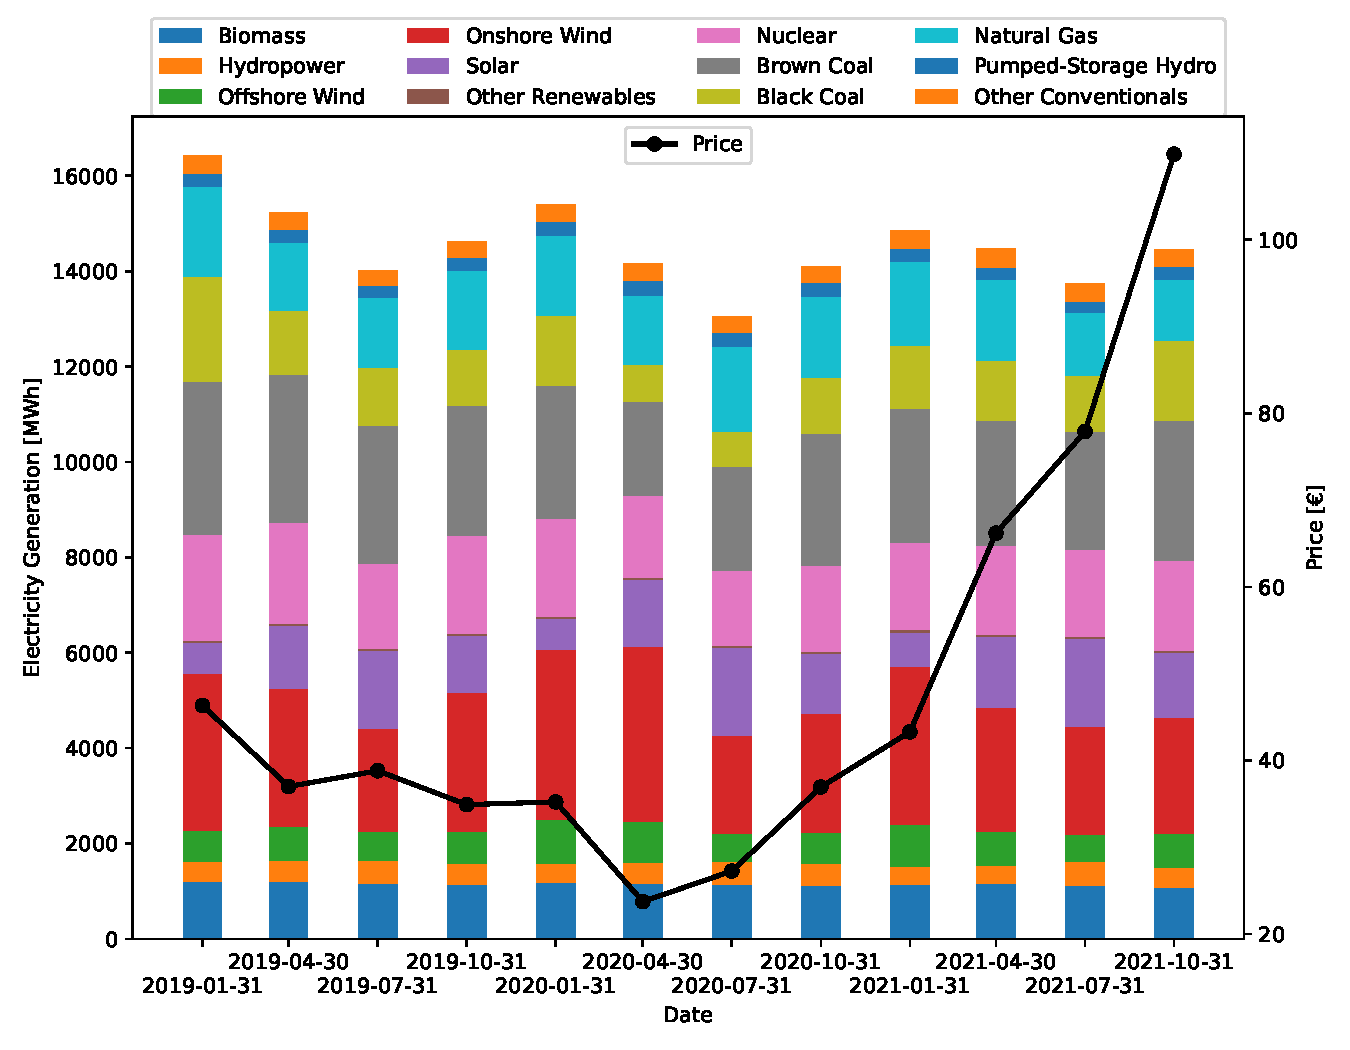
\includegraphics[width=\columnwidth]{doc/fig/quarterly_technology_mix_with_price.pdf}
    \caption{Quarterly electricity generation separated by source and spot prices from 2019 to 2021.}
    \label{fig:quarterly_mix}
\end{figure}
Figure \ref{fig:quarterly_mix} shows the relative contribution of the different electricity sources as well as the spot prices over each quarter from 2019 to 2021.
It is visible that the most important renewable sources are onshore and offshore wind as well as solar, while the largest conventional sources are brown coal and nuclear.
Moreover, market prices fall until the second quarter of 2020 to a minimum of 23.73 €/MWh, most likely due to the COVID-19 pandemic which reduced the demand and thereby depressed prices \citep{covid_electricity_systems}.
After the second quarter of 2020, the electricity prices rise significantly to a maximum of 109.88 €/MWh due to a multitude of factors, most notably an economic recovery causing demand shocks \citep{long_covid_energy_prices}. 
\begin{figure}[h]
    \centering
    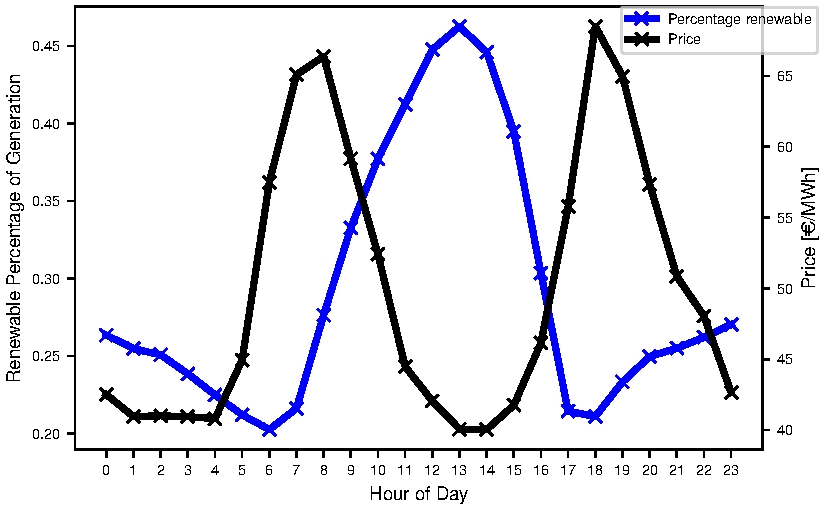
\includegraphics[width=\columnwidth]{doc/fig/example_day.pdf}
    \caption{Spot price and renewable share of generation on March 1, 2021.}
    \label{fig:example_day}
\end{figure}
Figure \ref{fig:example_day} shows the hourly electricity spot price and renewable share of generation over the duration of one exemplary day. 
It is visible that the price decreases when renewables generate more electricity and vice versa. 
% One can note that the contribution of the renewables increases between hour 8 and hour 17 during the day. 
% This can be attributed to the solar system, as it generates electricity only at daytime and reaches its peek at hour 13, where the sun is at its highest point causing the price to decrease. 

\section{Methods} \label{sec:methods}
We use a linear regression model to investigate the relationship between the spot price $p_t$ and the electricity generation $g_t$ at a time $t$ with an error of $\epsilon_t$:
$$
    p_t = \beta_0 + \beta_1\cdot g_t + \epsilon_t \quad \forall t,
$$
where the unknown parameters $\beta_0$ and $\beta_1$ represent the intercept and the slope of the fitted line, respectively \citep{Wasserman2004}.
To obtain the estimator we use an implementation provided by the library \enquote{scikit-learn} \citep{scikit-learn}.

% Regression analysis is a statistical technique for investigating and modeling the relationships between variables % \citep{montgomery2021introduction}. 

% In our case we have two variables: the price as the dependent variable, and the electricity generation as independet.
% If we let y represent the price and x represent electricity generation, then the equation of a straight line relating these two variables is 

% where $\beta_0$ is the intercept and $\beta_1$ is the slope.
% In other words, we want to estimte the spot prices from the electricity generation using a linear model.
% Depending on the slope of the regression line, we can conclude on the correlation of the two variables. 
%We will use this technique to analyze the renwable electricity generation as well as the conventional electricity generation.
%We will make the correlation of those variables visible and show the merit-order effect. 

% regression line conventional: y = 0.01067163 * x - 28.191637699817782
%    "              renewable:  y = - 0.00563317 * x + 91.00702286781541
% Can we conclude that conventional increases the price twice more than
% renewable decreases it? (|Slope_con| is nearly twice as big as |Slope_ren|)

\section{Results}
The data and analysis can be found on Github \citep{github_repo}.
We divide the sources into renewable and conventional and separately fit regression models as described in Section \ref{sec:methods} on the aggregated generation data:
\enquote*{Biomass}, \enquote*{hydropower}, \enquote*{onshore wind}, \enquote*{offshore wind}, \enquote*{solar}, and \enquote*{other renewables} are classified as renewable.
\enquote*{Nuclear}, \enquote*{brown coal}, \enquote*{black coal}, \enquote*{natural gas} and \enquote*{other conventionals} are classified as conventional.
% TODO: define renewable!
It is unclear where to situate pumped-storage hydro:
Storage unit operators do arbitrage in time in order to make a profit, i.e.\ they charge during times of low prices and discharge during times of high prices.
Thus, generation from pumped-storage hydro has a positive relationship with the market price.
On the one hand, due to the ability to control its output it could be attributed to the conventional sources.
On the other hand, times of low prices mostly coincide with high renewable generation, hence it shifts renewable sources in time.
For this reason we neglect pumped-storage hydro in the analysis.

Results of the regression analysis are displayed in Figure \ref{fig:ren_vs_con_regression}.
The opposite effect of renewable and conventional generation on market prices as described in Section \ref{sec:intro} is visible:
Renewable generation shows a negative relationship with prices, i.e.\ times of high generation coincide with low prices.
Conventional generation shows a positive relationship with prices, where prices are high during times of high generation.
High electricity prices in 2021 due to external effects could potentially lessen the visibility of the effect for renewable generation.

%\begin{itemize}
%    \item Figure \ref{fig:ren_vs_con_regression} shows the opposite effects of renewable and conventional electricity generation on the prices.
%    \item Data and analysis can be found on Github \citep{github_repo}.
%    \item Figure \ref{fig:pumped_hydro_regression} shows that generation from pumped-storage hydro has a positive relationship with the market price.
%    This is because operators of storage units do arbitrage in time in order to make a profit, i.e.\ they charge during times of low prices and discharge during times of high prices.
%    Thus, prices are generally higher when they are producing.
%\end{itemize}

%\begin{figure}[h]
    %\centering
    %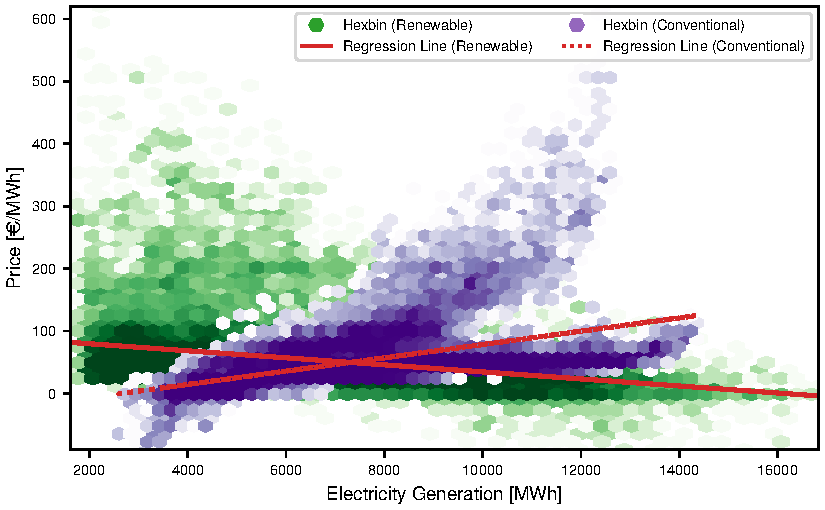
\includegraphics[width=0.8\columnwidth]{doc/fig/ren_vs_con_regression.pdf}
    %\caption{Caption}
    %\label{fig:ren_vs_con_regression}
%\end{figure}

\begin{figure}[h]
    \centering
    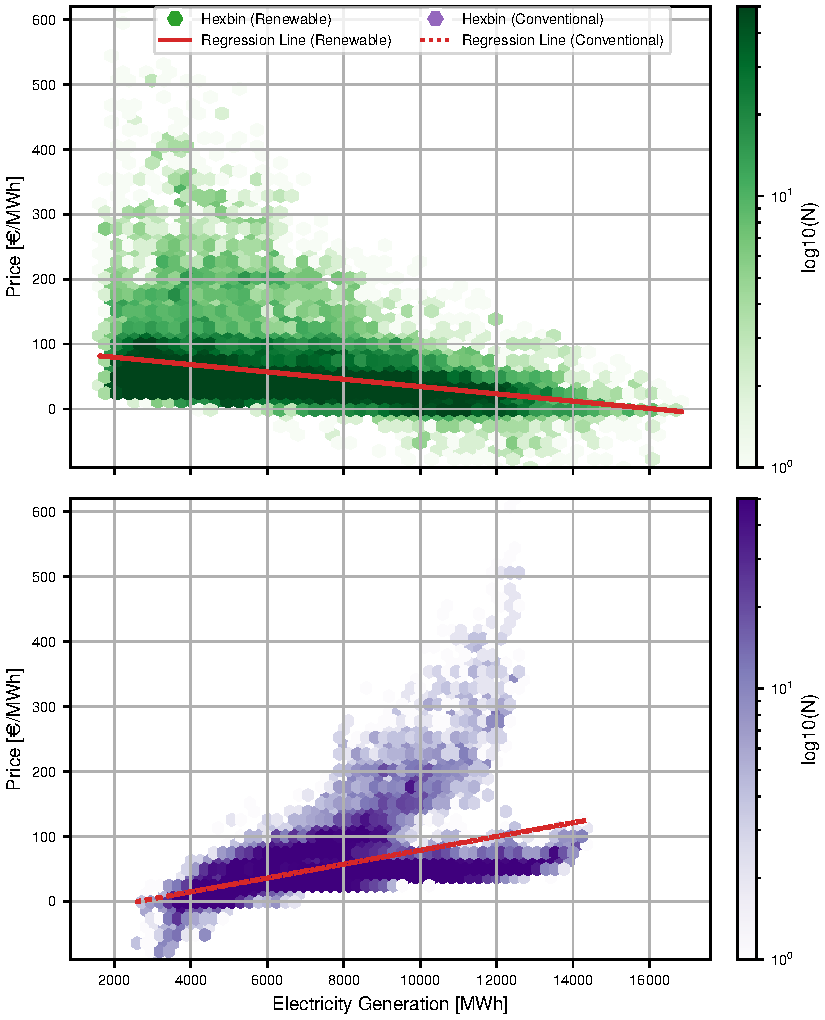
\includegraphics[width=\columnwidth]{doc/fig/ren_vs_con_regression_separate.pdf}
    \caption{Separate regression analyses relating renewable and conventional generation to spot market prices. Due to the large number of data points the data is aggregated into hexagons whose color intensity reflects the number of elements it contains.}
    \label{fig:ren_vs_con_regression}
\end{figure}

\section{Conclusion}
Due to the merit-order, an abundance of renewable electricity generation depresses market prices prices while conventional sources cause higher prices when they are needed, as the most expensive generator sets the price.
We investigate these effects using data from the years of 2019 to 2021 for Germany and Luxembourg compiled by the German Federal Network Agency, who receives it from transmission system operators and the European power exchange.
By splitting the electricity generation sources into renewable and conventional and then separately applying linear regression analysis, we are able to relate the generation to the market price and thereby show these opposite effects.

\bibliographystyle{plainnat}
\bibliography{literature}
\end{document}
